%% ------------------------------------------------------------------------- %%
\chapter{Experimento}
\label{cap:experimento}


Neste capítulo apresentaremos as etapas do processo de treinamento e avaliação das redes neurais. De acordo com \cite{nndesign:2014:pratical-training-issues}, o treinamento e avaliação de uma rede neural são compostas pelas seguintes etapas:
\begin{itemize}
    \item Coleta e pré-processamento dos dados
    \item Definição do tipo de rede neural e arquitetura
    \item Seleção do algoritmo de treinamento
    \item Treinamento
    \item Análise do desempenho da rede neural
    \item Utilização do modelo
\end{itemize}

Conforme a Figura~\ref{fig:training-neural-network-cyclic}, este é um processo cíclico e iterativo que inicia-se com a coleta e pré-processamento dos dados e termina com a utilização do modelo. Neste capítulo iremos apresentar as seguintes etapas deste processo:

\begin{itemize}
    \item Coleta e pré-processamento dos dados
    \item Treinamento
    \item Análise do desempenho da rede neural
\end{itemize}

E com relação as outras etapas, algumas já foram discutidas em outros capítulos ou estão fora do escopo do presente trabalho. A etapa de ''definição do tipo de rede neural e arquitetura'' já foi discutida no Capítulo~\ref{cap:abordagem} e a ''utilização do modelo'' está fora do escopo do trabalho neste momento. Em relação a etapa de ''seleção do algoritmo de treinamento'', optamos por fixar o algoritmo de otimização \emph{Adam} para aprendizagem, proposto por \cite{yao-2018}. 



\begin{figure}[H]
\centering
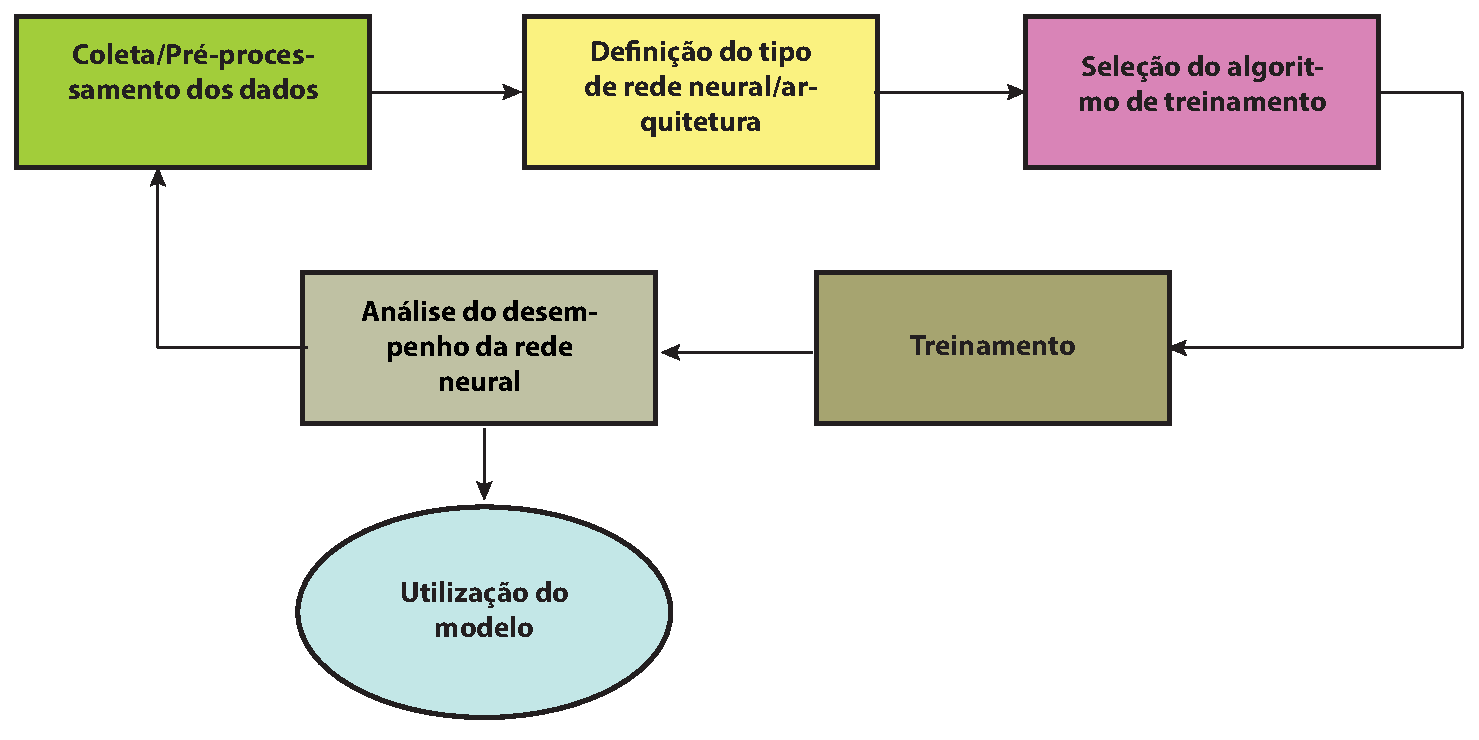
\includegraphics[width=1\textwidth]{figuras/cap-experimento/neural_network_training_lifecycle_dissertation.pdf}
\caption{Ilustração do processo de treinamento e avaliação de uma rede neural. Figura adaptada do \cite{nndesign:2014:pratical-training-issues}.} 
\label{fig:training-neural-network-cyclic}
\end{figure}

\section{Coleta e pré-processamento dos dados}
\label{sec:coleta-pre-processamento-dos-dados}

Conforme \cite{nndesign:2014:pratical-training-issues}, o processo de treinamento e avaliação de uma rede neural inicia-se com a coleta e pré-processamento dos dados. Em nosso caso, não houve coleta, pois utilizamos parte do conjunto de dados disponibilizados por \cite{yao-2018}. E estes dados estão sob a licença \href{https://creativecommons.org/licenses/by/4.0/}{Creative Commons}, onde o uso é permitido desde que faça referência ao trabalho dos pesquisadores. Ressaltamos que utilizamos parte do conjunto, pois os pesquisadores coletaram questões e trechos de código-fonte em Python e SQL do site \Gls{sof} e, em nosso trabalho, optamos apenas por utilizar o conjunto de dados em Python. 

 Uma peculiaridade desses dados em relação às amostras utilizadas em outros trabalhos \cite{iyer-etal-2016-summarizing, Allamanis-bimodal-source-code-natural-language:2015}, é o fato de conter ''apenas'' questões do tipo \textit{how-to-do-it}. As respostas para este tipo de questão costumam ser mais diretas e ter apenas um trecho de código-fonte como solução \citep{yao-2018}. Além disso, conforme apontado por \cite{cambronero-deep-learning-code-search:2019}, as questões coletadas em fóruns abertos de perguntas e respostas de programação costumam expressar mais as intenções do desenvolvedor quando comparadas com comentários \gls{docstring}, por exemplo. Esta característica vai  ao encontro com a nossa definição adotada para o problema de \textit{code retrieval}, onde pretendemos encontrar uma semântica para o trecho de código-fonte, de forma que atenda às intenções de busca do desenvolvedor. Para isto, um caminho é ensinar um modelo a associar trechos de código-fonte a questões que expressem as intenções do desenvolvedor.

\subsection{Conjunto de dados}
\label{sec:conjunto-dados}

O conjunto de dados disponibilizado por \cite{yao-2018} é formado por $\bm{147.546}$ pares de questões em inglês e trechos de código-fonte em Python e $\bm{119.519}$ em SQL. Eles foram coletados do site \Gls{sof} e contemplam questões do ano de 2008 a 2016\footnote{\url{https://github.com/LittleYUYU/StackOverflow-Question-Code-Dataset}}. Podemos dividi-los em 3 (três) subconjuntos distintos:

\begin{itemize}
    \item N1: Questões coletadas do \Gls{sof} que continham apenas um trecho de código-fonte na descrição da resposta
    \item N2: Questões que apresentavam mais de um trecho de código-fonte na descrição
    \item N3: Pares de questões e trechos de código-fonte anotados manualmente
\end{itemize}



\begin{figure}[H]
\centering
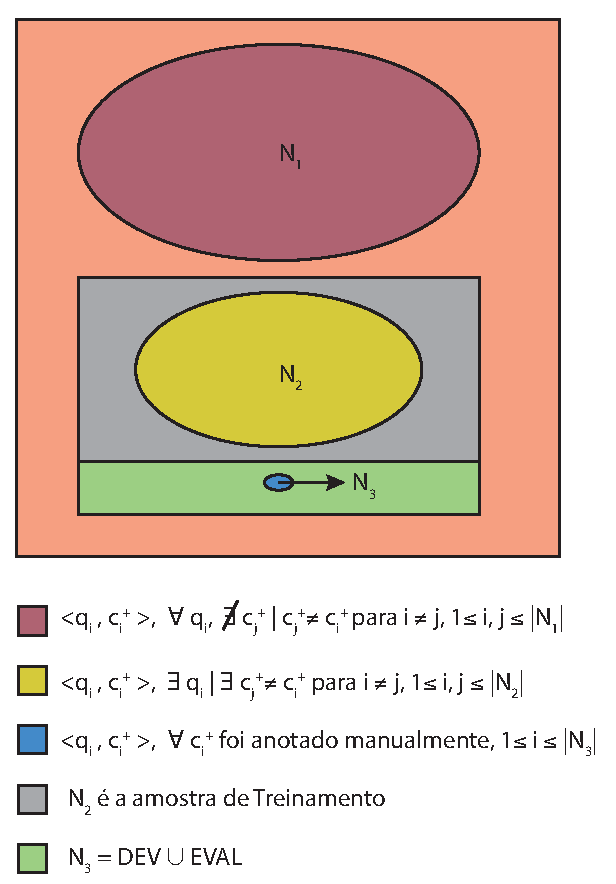
\includegraphics[width=0.6\textwidth]{figuras/cap-experimento/distinct-subsets-yao-sample.pdf}
\caption{Divisão das amostras de pares de questões e trechos de código disponibilizados por \cite{yao-2018}: $N_{1} = \{(q_{i}, c_{i}^{+})\;,\; \forall\; q_{i},\;\nexists\; c_{j}^{+}\; |\; c_{j}^{+} \neq c_{i}^{+}\; \text{para}\; i \neq j,\; 1 \leq i,j \leq |N_{1}| \}$, $N_{2} = \{(q_{i}, c_{i}^{+})\;,\; \exists\; q_{i}\; | \;\exists\; c_{j}^{+} \neq c_{i}^{+}\; \text{para} \; i \neq j,\; 1 \leq i,j \leq |N_{2}| \}$, $N_{3} = \{(q_{i}, c_{i}^{+}),\; \forall\; c_{i}^{+} \text{foi anotado manualmente}, 1 \leq i \leq |N_{3}| \}$. Onde $N_{1} \cap N_{2} \cap N_{3} = \varnothing$, $q_{i} \in \mathbb{Q}$ e $c_{i}^{+},  c_{j}^{+} \in \mathbb{C}$. E $c_{i}^{+}, c_{j}^{+}$ são respostas anotadas como corretas. $\mathbb{Q}$ e $\mathbb{C}$ representam o conjunto de questões e trechos de código respectivamente.} 
\label{fig:distinct-subset-python-pair-question-code}
\end{figure}

A ilustração da divisão dos subconjuntos pode ser visualizada na Figura~\ref{fig:distinct-subset-python-pair-question-code}. Um ponto importante a ser ressaltado, são os casos em que há mais de um trecho de código-fonte na descrição da resposta, pois nem todo trecho é necessariamente uma solução para a questão. No exemplo a seguir, os trechos \emph{T2} e \emph{T4} não são soluções para a dúvida do usuário. O trecho \emph{T2} apenas inicializa um array e o trecho \emph{T4} mostra a saída do comando \textit{print} para o vetor já convertido\footnote{Site: \url{https://stackoverflow.com/questions/34349762/convert-2d-numpy-array-to-string} Esta questão apresenta 6 trechos de código-fonte, mas para melhor visualização, optamos por colocar apenas 4 trechos em nosso exemplo\label{foot:exemplo-stackoverflow-mais-de-um-trecho}}.



\begin{tcolorbox}[colframe=orange!75!black,colback=gray!15!white,fonttitle=\bfseries,adjusted title=\large{Título da questão: convert 2d numpy array to string}~\ref{foot:exemplo-stackoverflow-mais-de-um-trecho}]
\begin{mypythongreen}{Trecho T1: A one-liner will do:}
b = '\n'.join('\t'.join('%0.3f' %x for x in y) for y in a)
\end{mypythongreen}

\begin{mypythonred}{Trecho T2: Using a simpler example:}
>>> a = np.arange(25, dtype=float).reshape(5, 5)
>>> a
array([[  0.,   1.,   2.,   3.,   4.],
       [  5.,   6.,   7.,   8.,   9.],
       [ 10.,  11.,  12.,  13.,  14.],
       [ 15.,  16.,  17.,  18.,  19.],
       [ 20.,  21.,  22.,  23.,  24.]])
\end{mypythonred}
\begin{mypythongreen}{Trecho T3: is equivalent to:}
res = []
for y in a:
    res.append('\t'.join('%0.3f' %x for x in y))
b = '\n'.join(res)
\end{mypythongreen}
\begin{mypythonred}{Trecho T4: prints this:}
0.000   1.000   2.000   3.000   4.000
5.000   6.000   7.000   8.000   9.000
10.000  11.000  12.000  13.000  14.000
15.000  16.000  17.000  18.000  19.000
20.000  21.000  22.000  23.000  24.000
\end{mypythonred}
\end{tcolorbox}


Para diferenciar os trechos de código presentes em uma mesma resposta, \cite{yao-2018} anotaram os pares com $\bm{1}$, quando o trecho é solução para a pergunta e $\bm{0}$, caso contrário. Inicialmente foi feita uma anotação manual em uma amostra de aproximadamente 2000 pares. E posteriormente, uma rede neural recorrente foi treinada a classificar os trechos de código que são soluções para as perguntas, obtendo um resultado de F1 de $0,916$ e acurácia de $0,911$ em seus testes. Ao final, os pesquisadores utilizaram este modelo para classificar automaticamente o conjunto de pares $N_{2}$ e disponibilizaram os dados anotados e divididos conforme a Tabela~\ref{table:summary-training-data-yao-staqc}.

\begin{table}[h]
\centering
\begin{tabular}{ p{16em} P{10em} P{10em} }
\hline
  & \multicolumn{2}{c}{\textbf{Questão}}\\
\hline
\textbf{Código-fonte} & \textbf{Python} & \textbf{SQL}  \\
\hline

$N_{1}$: Apenas 1 trecho de código na descrição da resposta & $85.294$ & $75.637$ \\

$N_{2}$: Trechos de código-fonte anotados automaticamente & $60.083$ & $41.826$ \\

$N_{3}$: Trechos de código-fonte anotados manualmente & $2.169$ & $2.056$  \\

 \hline
 \textbf{Total} & $\bm{147.546}$ & $\bm{119.519}$\\
 \hline 
 
\end{tabular}
\caption{Divisão do conjunto de dados disponibilizado por \cite{yao-2018}. O conjunto formado por "Trechos de código-fonte anotados automaticamente" contém questões que tem mais de um trecho de código-fonte por resposta. Quando há mais de um trecho de código-fonte por resposta, nem todo trecho é uma solução. Neste caso, \cite{yao-2018} criaram um framework para anotá-los automaticamente. Eles obtiveram F1 de $0,916$ e acurácia de $0,911$ em seus testes de classificação automática das respostas corretas.}
\label{table:summary-training-data-yao-staqc}
\end{table}

\subsection{Conjunto de dados para avaliação e treinamento}
\label{sec:conjunto-dados-avaliacao-treinamento}

Para avaliar a dificuldade do problema, analisamos a quantidade de palavras presentes nas questões e trechos de código-fonte das amostras utilizadas no treinamento e avaliação dos nossos modelos. Para o treinamento, optamos por utilizar o conjunto $N_{2}$, pois ele apresenta uma variabilidade maior, já que em torno de 27\% das questões contém mais de um trecho de código-fonte anotados como correto, ou seja, 27\% das perguntas tem mais de uma opção de solução. No caso da avaliação, utilizamos o conjunto $N_{3}$, que apresenta uma maior qualidade e acurácia nos dados, pois eles foram anotados manualmente. A quantidade de pares presentes nas amostras $N_{2}$ e $N_{3}$ podem ser visualizadas na Tabela~\ref{table:divisao-amostras}. Lembrando que $N_{3} = DEV \cup EVAL$. E $N_{2} \cap N_{3} = \varnothing$.

\begin{table}[h]
\centering
\begin{tabular}{ p{5cm} r  }
 \hline
 \textbf{Amostras} & \textbf{Quantidade de pares $<q_{i}, c_{i}^{+}>$}\\
 \hline
 $N_{2} = \text{Treinamento}$ & $60.083$\\
 
 $N_{3} \supset \text{DEV}$ & $1.085$ \\
 
 $N_{3} \supset \text{EVAL}$ & $1.084$\\
 \hline
 \textbf{Total} & $\bm{62.252}$\\
 \hline
\end{tabular}
\caption{Divisão das amostras para treinamento e avaliação. O conjunto de dados é formado por pares $<q_{i}, c_{i}^{+}>$, onde $q_{i}$ é uma questão e $c_{i}^{+}$ é um trecho de código-fonte anotado como correto. O conjunto formado por pares anotados manualmente foi dividido em DEV e EVAL conforme o procedimento descrito por \cite{iyer-etal-2016-summarizing}. É possível visualizar uma ilustração deste procedimento nas Figuras \ref{fig:evaluation-process} e \ref{fig:final-evaluation-process}.}
\label{table:divisao-amostras}
\end{table}


De acordo com a Tabela~\ref{table:statistical-descriptive-of-pythons-sample}, as questões tem aproximadamente em média $9$ palavras com um desvio padrão de $\pm 3.71$. Já os trechos de código apresentam aproximadamente uma média de $44$ e um desvio padrão de $\pm 49$. O valor alto do desvio padrão para os trechos de código é um indicativo de maior variabilidade da quantidade de palavras. Este valor da média e desvio padrão alto podem ser influenciados por pontos fora da curva também, i.e., trechos de código com uma enorme quantidade de palavras. Para entender um pouco melhor como está distribuída esta quantidade, apresentamos os percentis na Tabela~\ref{table:statistical-descriptive-of-pythons-sample} e o diagrama de caixa com os respectivos quartis na Figura~\ref{fig:boxplot-number-of-words}.

\begin{table}[h]
\centering
\begin{tabular}{ p{5em} P{4em} P{4em} P{4em} P{4em} P{4em} P{4em} }
\hline
  & \multicolumn{5}{c}{\textbf{Quantidade de palavras}}\\
\hline
 & \textbf{$\mathbf{N_{2}}$\_Q} & \textbf{$\mathbf{N_{2}}$\_C} & \textbf{Dev\_Q} & \textbf{Dev\_C} & \textbf{Eval\_Q} & \textbf{Eval\_C}  \\
\hline

Média &	 $8.89$ & $44.41$ &	 $9.15$ & $44.31$ &	 $9.35$ & $42.78$ \\

Desvio padrão & $3.65$ & $55.19$ &	 $3.64$ & $51.87$ &	 $3.85$ & $43.82$ \\

Mínimo & $2$ & $1$ &	 $3$ & $1$ &	 $3$ & $2$ \\ 

25\% & $6$ & $16$ &	 $7$ & $15$ &	 $6$ & $15$ \\

50\% & $8$ & $30$ &	 $9$ & $29$ &	 $9$ & $29$ \\

75\% & $11$ & $54$ &	 $11$ & $52$ &	 $11$ & $55$ \\

Máximo & $32$ & $3566$ &	 $25$ & $708$ &	 $27$ & $439$ \\
 
 
 \hline 
 
\end{tabular}
\caption{Estatística descritiva da quantidade de palavras nas amostras de questões e trechos de código em Python utilizados no treinamento e avaliação dos modelos. O prefixo $\mathbf{N_{2}}$ refere-se a amostra de treinamento, conforme a Figura~\ref{fig:distinct-subset-python-pair-question-code}. Os prefixos \textbf{Dev} e \textbf{Eval} referem-se a amostra para escolha do modelo e a amostra para avaliação final conforme procedimento ilustrado nas Figuras \ref{fig:evaluation-process} e \ref{fig:final-evaluation-process}. Os sufixos \textbf{Q} e \textbf{C} referem-se ao conjunto de palavras das questões e trechos de código-fonte respectivamente. Esta tabela inclui a média, desvio padrão e os percentis 25\%, 50\% e 75\% após o pré-processamento. Os detalhes sobre o pré-processamento estão presentes na Seção~\ref{sec:pre-processamento}.}
\label{table:statistical-descriptive-of-pythons-sample}
\end{table}

Tanto pela Tabela~\ref{table:statistical-descriptive-of-pythons-sample} quanto pela Figura~\ref{fig:boxplot-number-of-words}, podemos verificar que as questões apresentam um variabilidade e quantidade menor de palavras. Aproximadamente 50\% das questões tem em torno de $6$ a $11$ palavras. Enquanto os trechos de código apresentam 50\% das vezes a quantidade aproximada de $15$ a $54$ palavras. A partir destas informações, podemos dizer que as nossas amostras são constituídas por questões relativamente curtas e trechos de código que variam de 1 (uma) a 3 (três) sentenças de tamanho em linguagem natural \citep{casi-newell-sentence-length-2018}. Aparentemente, essa amostra não trará muitas dificuldades à aprendizagem por parte das redes convolucionais, pois as redes convolucionais priorizam as interações locais e tem dificuldade em correlacionar palavras muito distantes em uma sentença, o que não é o nosso caso.



\begin{figure}[h]
\centering
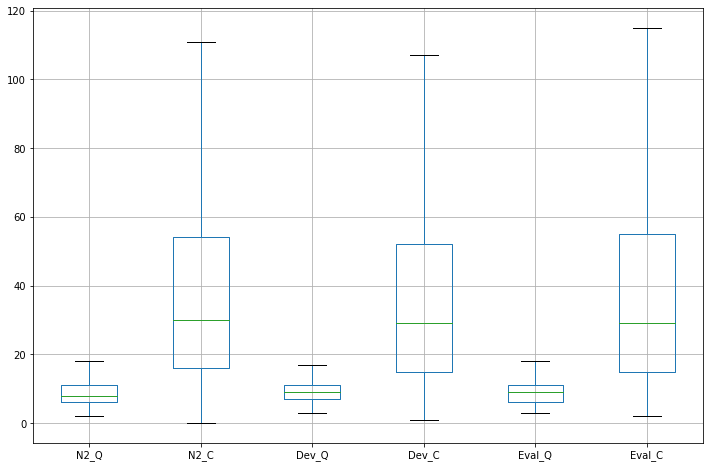
\includegraphics[width=1\textwidth]{figuras/cap-experimento/boxplot_number_of_words.png}
\caption{Diagrama de caixa para visualizar graficamente a distribuição da quantidade de palavras das questões e trechos de código-fonte por meio de quartis. Este diagrama de caixa exibe o Q1 (primeiro quartil), Q2 (segundo quartil) e Q3 (terceiro quartil). Eles referem-se aos percentis 25\%, 50\% e 75\% da Tabela~\ref{table:statistical-descriptive-of-pythons-sample}. O segundo quartil (Q2) refere-se a mediana. }. 
\label{fig:boxplot-number-of-words}
\end{figure}

\subsection{Pré-processamento}
\label{sec:pre-processamento}

O pré-processamento é a primeira etapa a ser realizada após a coleta dos dados e o objetivo é transformá-los e/ou adaptá-los para atender aos requisitos de entrada do modelo e/ou facilitar a aprendizagem durante o treinamento. Em nosso trabalho, utilizamos dois procedimentos com o intuito de facilitar a aprendizagem das redes neurais:

\begin{itemize}
    \item Substituição dos literais numéricos e textuais dos trechos de código-fonte
    \item Representação das palavras através de um vetor de representação distribuída
\end{itemize}

Para diminuir a dispersão dos dados, substituimos os literais númericos e textuais por palavras \emph{''NUMBER''} e \emph{''STRING''}, e também as variáveis pela palavra \emph{''VAR''}. Para isto, utilizamos uma função disponibilizada por \cite{yao-2018} que percorre a árvore sintática do trecho do código-fonte em Python e realiza estas substituições. Além disso, utilizamos a função de \textit{tokenização} da biblioteca \Gls{keras} para transformar as questões e trechos de código-fonte em vetores numéricos, remover os caracteres especiais e tornar todas as palavras minúsculas. Os caracteres especiais removidos podem ser visualizados no código a seguir, através do parâmetro \textit{filters} no construtor da classe \textit{Tokenizer}.

\begin{mypythonembedding}{Construtor da classe \textit{Tokenizer} da biblioteca \textit{Keras}.}
Tokenizer(filters='!"#$%&()*+,-./:;<=>?@[\\]^_`{|}~\t\n', lower=True, split=' ')
\end{mypythonembedding}


Para auxiliar a aprendizagem das redes neurais, as palavras que compõem as questões e os trechos de código-fonte foram representados por um vetor de representação distribuída. Segundo \cite{Goodfellow-et-al-2016:representation-learning}, os vetores de representação distribuída induzem a um rico espaço de similaridade, no qual conceitos semanticamente similares estão próximos, facilitando a generalização e aprendizagem das redes neurais. Para mapear as palavras para vetores de representação distribuída, utilizamos o algoritmo \textit{word2vec} com \textit{skip-gram}. Segundo \cite{mikolov2013distributed}, \textit{skip-gram} obteve um bom desempenho em problemas semânticos, e.g., relacionar nomes de cidades a país, aproximar uma palavra masculina à sua palavra correspondente feminina. Essa é uma característica importante, pois irá auxiliar as redes neurais a diferenciarem instruções de decisão (\textit{if, else, elif}) de instruções de repetição (for, while), por exemplo. 

Conforme apontado no Capítulo~\ref{cap:abordagem}, mapeamos cada palavra presente nas questões e trechos de código-fonte para uma matriz única $\bm{T_{v}}^{|V| X 100}$, onde $|V|$ é o tamanho do vocabulário formado pelas palavras presentes nas questões e trechos de código-fonte e $100$ é a dimensão do vetor. Para ilustrar o conceito de vetor de representação distribuída e este rico espaço de similaridade, onde conceitos semanticamente similares estão próximos, criamos a Figura~\ref{fig:tsne-code-snippet-python} utilizando a ferramenta t-SNE, que permite visualizar dados de dimensão elevada \citep{scikit-learn-tsne-2019, quora-tsne-2019}. Nessa figura exibimos os vetores de representação distribuída das 66 palavras mais frequentes do vocabulário $\bm{V}$ e podemos notar as similaridades entre as palavras \emph{file}, \emph{open}  e \emph{write}, assim como \emph{set}, \emph{dict} e \emph{list}, devido a proximidade entre elas.

\begin{figure}[H]
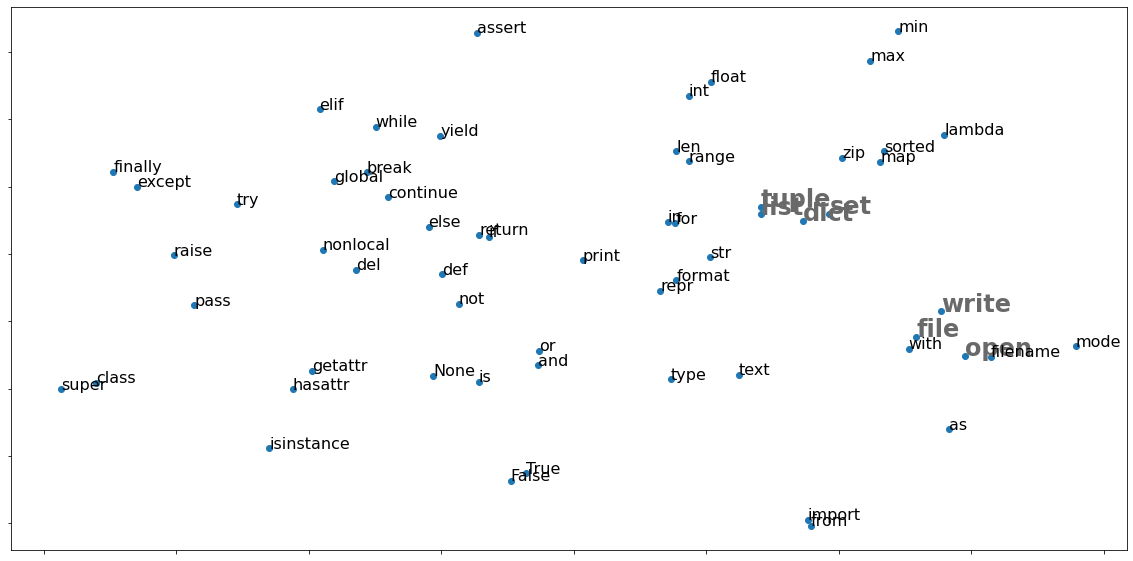
\includegraphics[width=1\textwidth]{figuras/cap-experimento/code_tsne.png}
\caption{Representação em 2D do vetor de representação distribuída de trechos de código-fonte. Imagem gerada através da ferramenta t-SNE. O vetor de representação distribuída foi criado a partir da amostra de pares de questões e trechos de código-fonte em Python disponibilizada por \cite{yao-2018}. Vetor criado utilizando o \textit{word2vec} com o algoritmo \textit{skip-gram} e o parâmetro \textit{window} com o valor $5$.}
\label{fig:tsne-code-snippet-python}
\end{figure}

\section{Treinamento}
\label{sec:treinamento}

Após as etapas de coleta de dados e pré-processamento, a próxima etapa é a de treinamento. Durante a etapa de treinamento que o nosso modelo irá aprender a correlacionar os trechos de código-fonte às questões. Para isto, o modelo irá treinar durante várias épocas com o objetivo de minimizar a função de custo. No nosso caso, a função de custo é a função de perda \textit{hinge}. Conforme citado na Seção~\ref{sec:funcao-objetivo}, o objetivo dessa função é induzir o nosso modelo a classificar os trechos de código-fonte anotados como corretos com uma pontuação maior que os trechos de código-fonte incorretos. A cada época, o algoritmo de otimização atualiza os pesos do modelo a fim de encontrar o conjunto ótimo de pesos que minimize a função de custo e permita o nosso modelo classificar corretamente os trechos de código-fonte às suas questões.

Para realizar a etapa de treinamento, algumas decisões foram tomadas. Listamos a seguir os principais pontos pelos quais tomamos decisão:

\begin{itemize}
    \item Divisão da amostra de treinamento e validação
    \item Duração do treinamento e critério de parada
    \item Critério de seleção do modelo
    \item Função objetivo
\end{itemize}



\begin{table}[h]
\centering
\begin{tabular}{ | p{5cm} | p{10cm} |  }
\hline
\textbf{Item} & \textbf{Decisão} \\
\hline
 Divisão da amostra de treinamento e validação & Utilizamos o conjunto $N_{2}$ composto por $60.083$ pares de questões e trechos de código-fonte. Durante o treinamento, do total de $60.083$ amostras, $42.058$ foram utilizadas para o conjunto de treinamento e $18.025$ para o conjunto de validação\\


\hline
 
Duração do treinamento e critério de parada & O modelo é treinado durante 500 épocas. Caso o valor da função de perda \textit{hinge} na amostra de treinamento fique abaixo de $0,0001$ ou o valor da função de perda na amostra de validação não diminua após 25 épocas consecutivas, o treinamento é interrompido\\

 \hline
Critério de seleção do modelo & \gls{one-hot-encoding} para questão e código-fonte \\
 
 & Combinou os vetores usando \acrshort{lstm} com \gls{mecanismo-atencao}\\
 
 \hline
 
 \multirow{2}{8em}{\cite{Gu-deep-code-search:2018}} & \textit{word2vec} para questão e código-fonte\\
 
 & Combinou os vetores usando uma rede bi-\acrshort{lstm}\\
 
 \hline
 
 \multirow{2}{8em}{\citep{Sachdev-neural-code-search:2018}} & \textit{word2vec} para código-fonte e questão\\
 
 & Combinou os vetores de \textit{tokens} da questão usando a média / Combinou os vetores do código-fonte através do \acrshort{tf-idf} \\
 
 \hline
 
 \multirow{2}{8em}{\cite{cambronero-deep-learning-code-search:2019}} & \textit{word2vec} para questões e código-fonte \\
 
 & Combinou os vetores de cada palavra da questão calculando a média / Combinou os vetores do código-fonte usando o \gls{mecanismo-atencao}\\
 
 \hline
 
\end{tabular}
\caption{Sumário das diferentes abordagens adotadas pelos pesquisadores para o problema do \textit{code retrieval}. Tabela adaptada de \cite{cambronero-deep-learning-code-search:2019}}
\label{table:training-decisions}
\end{table}


Adotamos o mesmo procedimento de treinamento proposto por \cite{iyer-etal-2016-summarizing}.  Para escolha do modelo e avaliação final, foi utilizado o conjunto $N_{3}$ de dados anotados manualmente. A divisão das amostras para treinamento e avaliação podem ser visualizadas na Tabela~\ref{table:divisao-amostras}. 

O procedimento de treinamento utilizado foi: . A cada época, o modelo é avaliado na amostra \emph{DEV}. O intuito desta avaliação é obter o melhor modelo conforme a métrica \acrshort{mrr}. A ilustração deste procedimento pode ser visualizado na Figura~\ref{fig:evaluation-process}.

\begin{figure}[p]
\centering
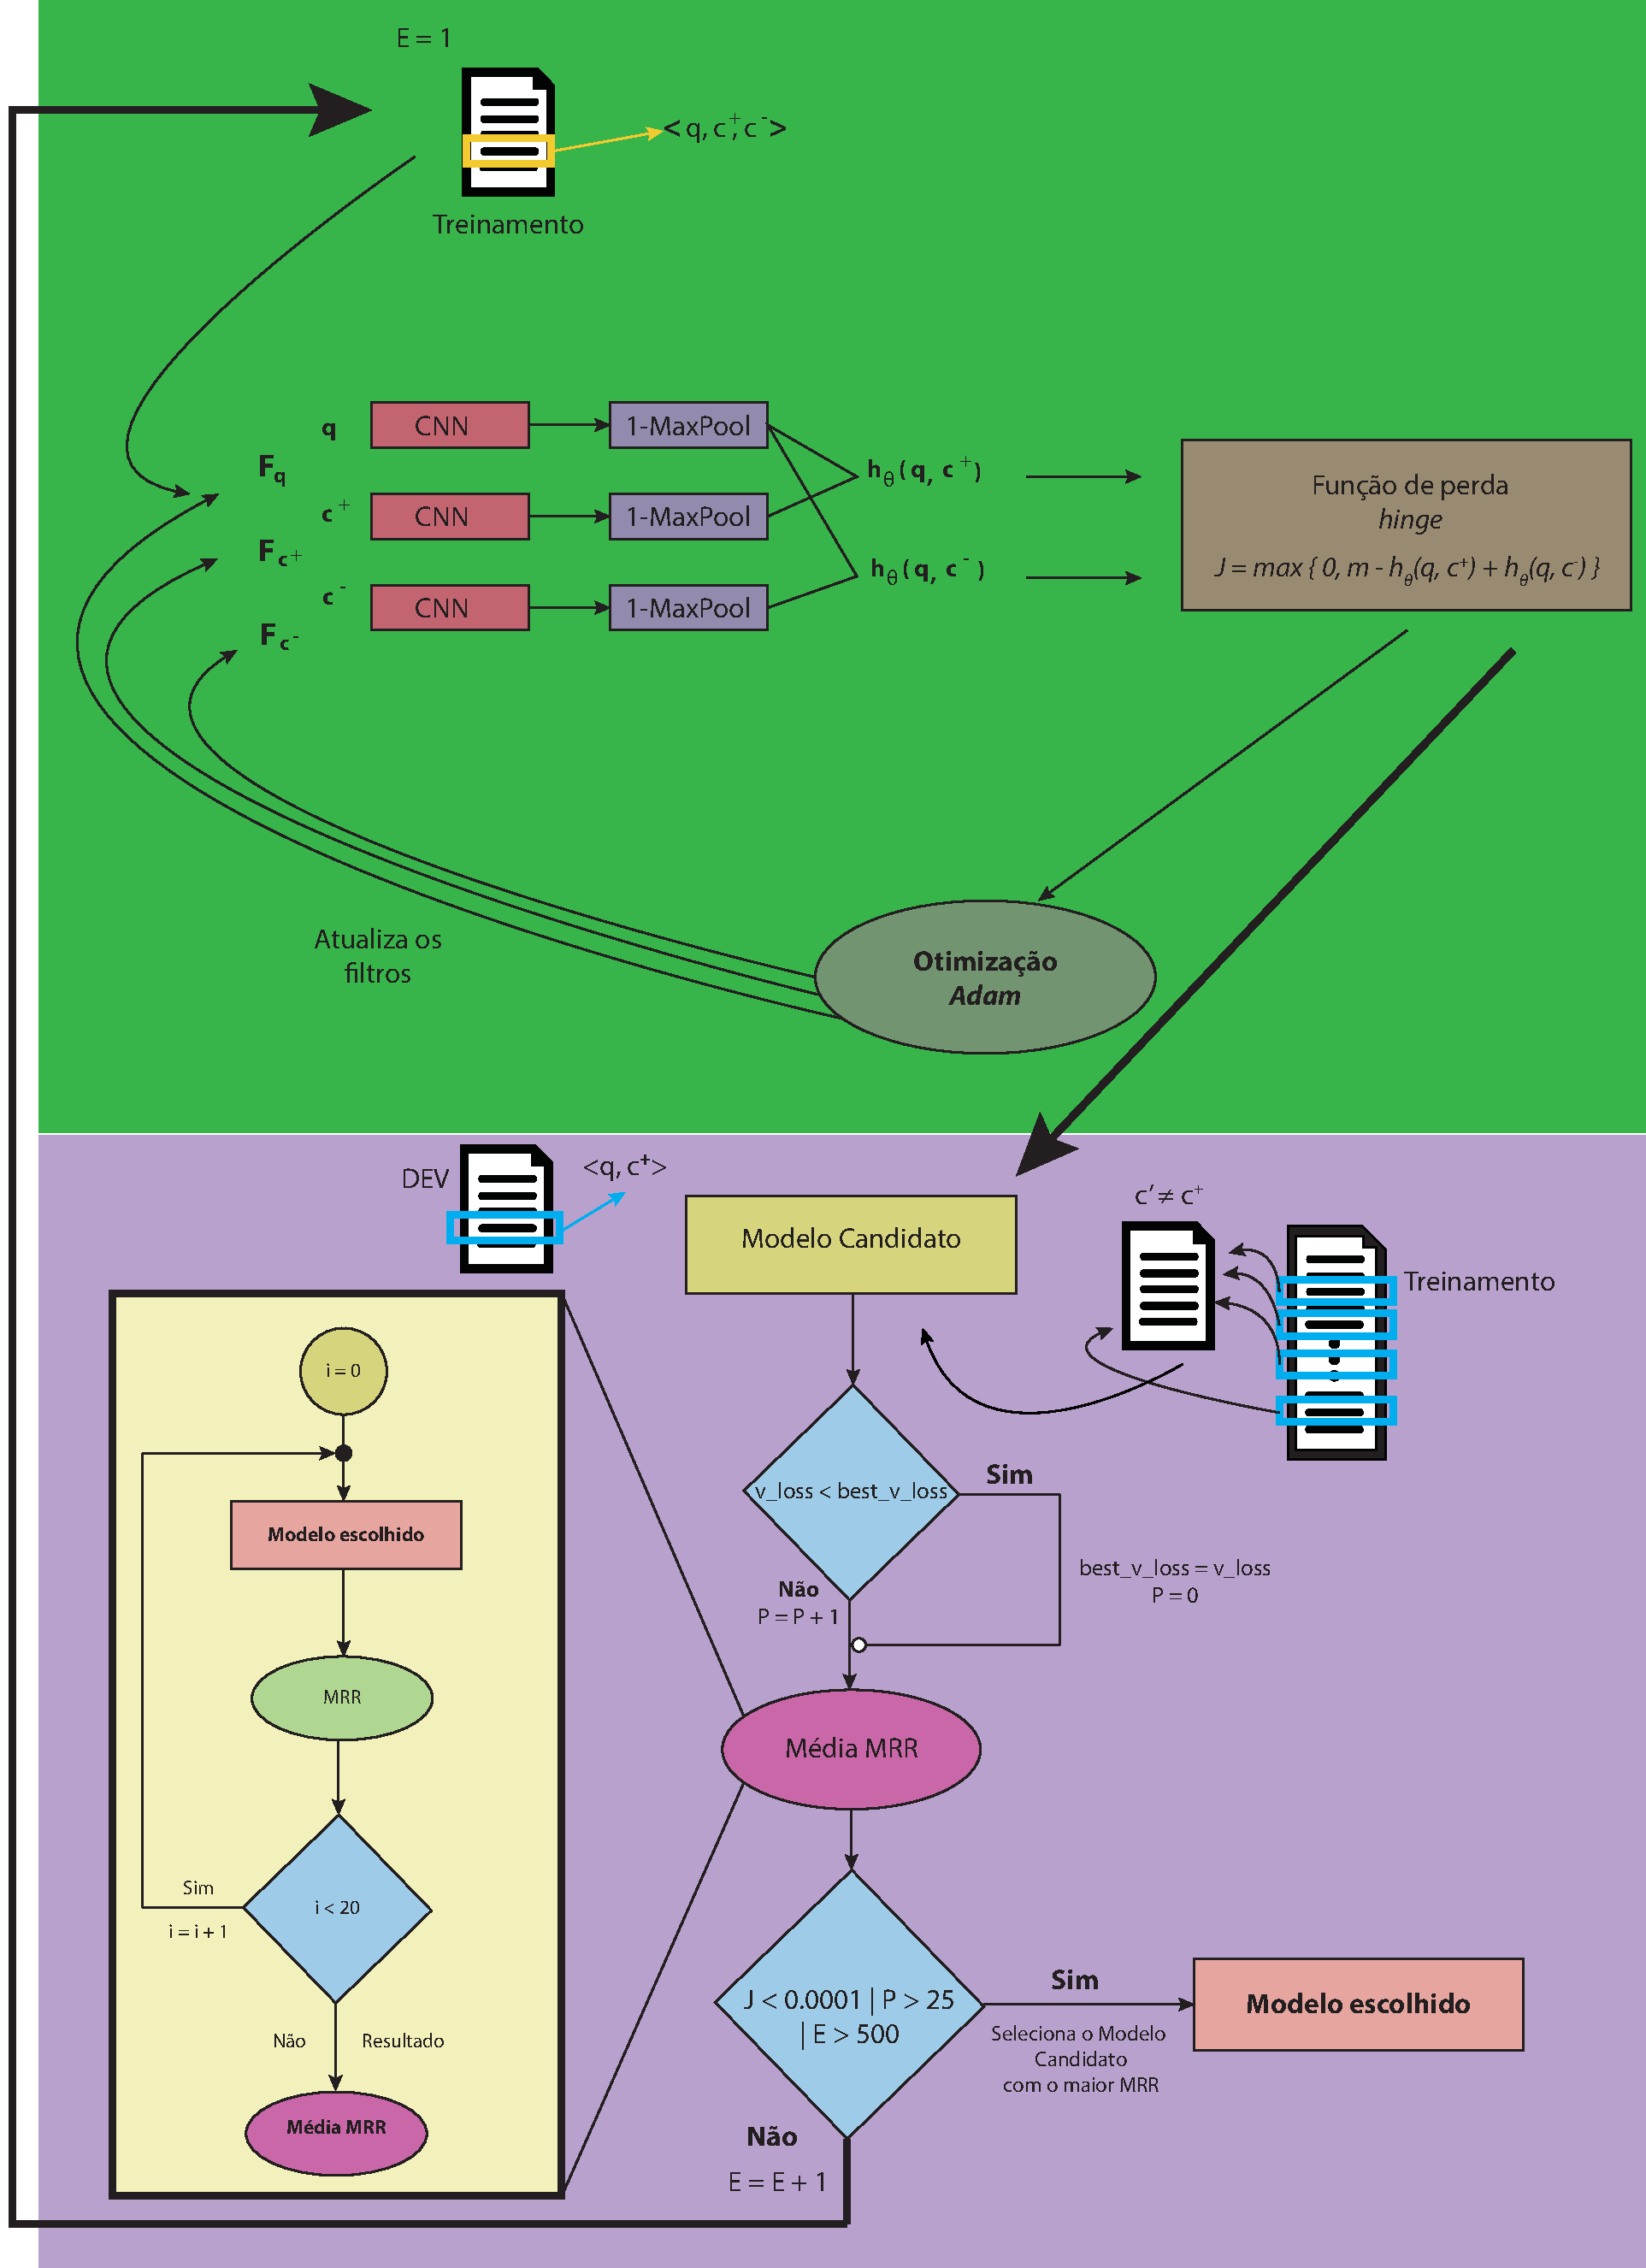
\includegraphics[height=1.3\textwidth]{figuras/cap-experimento/evaluation_process.pdf}
\caption{Ilustração do exemplo de treinamento de uma rede convolucional. Este procedimento é o mesmo adotado por \cite{iyer-etal-2016-summarizing}. $E$ é uma variável de controle para armazenar a quantidade de épocas. $P$ refere-se a quantidade de iterações seguidas em que não há diminuição do resultado da função de perda na amostra de validação. Os vetores de entrada dos modelos durante o treinamento são os vetores de representação distribuída $q, c^{+}, c^{'} \in \mathbb{R}^{150 X d}$, onde $150$ é o tamanho fixo dos vetores e $d$ é a dimensão do vetor. $F \in \mathbb{R}^{k X d}$ é o filtro convolucional, onde $k$ é o tamanho da janela e $d$ a dimensão do vetor. $h_{\theta}$ é a função \textit{cosine} de similaridade, $J$ é a função de perda \textit{hinge} e $m$ é a margem. O procedimento de treinamento está descrito na seção~\ref{sec:treinamento}.}
\label{fig:evaluation-process}
\end{figure}

Para cada par $<q_{i}, c_{i}^{+}>$ da amostra \emph{DEV}, onde $q_{i}$ uma questão e $c_{i}^{+}$ uma questão anotada como correta. Outros 49 distratores $c'$ são selecionados aleatoriamente da amostra de treinamento, tal que $c_{i}^{+} \neq c'$. Para cada questão, o modelo calcula a similaridade entre a questão e os trechos de código-fonte. O cálculo de similaridade é feito através da função $h_{\theta}$, onde $h_{\theta}$ é a função \textit{cosine}. 

Posteriormente, os trechos de código-fonte são ordenados de forma decrescente, do mais similar (maior pontuação) ao menos similar (menor pontuação). Com os trechos ordenados, obtém-se a posição do trecho $c_{i}^{+}$ para cálculo do \textit{reciprocal rank}. \textit{Reciprocal rank} é o inverso da posição da primeira ocorrência de $c_{i}^{+}$ encontrada no resultado. Com o \textit{reciprocal rank}, calcula-se o \acrshort{mrr}. \acrshort{mrr} é a média do \textit{reciprocal rank} para a amostra inteira \citep{Gu-deep-code-search:2018}:

\begin{equation}\label{eq:mrr}
MRR = \frac{1}{n} * \sum_{i = 1}^{n}\frac{1}{p_{i}^{+}}    
\end{equation}

Onde $n$ é a quantidade de questões presentes na amostra, $p_{i}^{+}$ é a posição da primeira ocorrência do trecho $c_{i}^{+}$ entre os trechos ordenados. 

Este procedimento é repetido durante 20 iterações. A cada iteração, outros 49 distratores são selecionados e, ao final, obtém-se a média \emph{MRR} do modelo. Basicamente, a cada época verificamos o resultado MRR do modelo comparando a resposta anotada como correta com outros 49 distratores. E selecionamos o modelo que obtiver a melhor média MRR. Este modelo escolhido será utilizado na avaliação final.





\section{Análise do desempenho da rede neural}
\label{sec:analise-do-desempenho-da-rede-neural}

\subsection{Avaliação}
\label{sec:avaliacao}

A avaliação final na amostra \emph{EVAL} utiliza o mesmo procedimento da amostra \emph{DEV} descrito anteriormente. Quer dizer, calculamos o MRR para cada par $<q_{i}, c_{i}^{+}>$ da amostra \emph{EVAL} juntamente com outros 49 distratores $c'$ que são selecionados aleatoriamente da amostra de treinamento, tal que $c_{i}^{+} \neq c'$. Este procedimento de cálculo do MRR é repetido durante 20 iterações. Após as 20 iterações, obtemos a média final do nosso modelo. A ilustração deste procedimento pode ser visualizada na Figura~\ref{fig:final-evaluation-process}.

\begin{figure}[h]
\centering
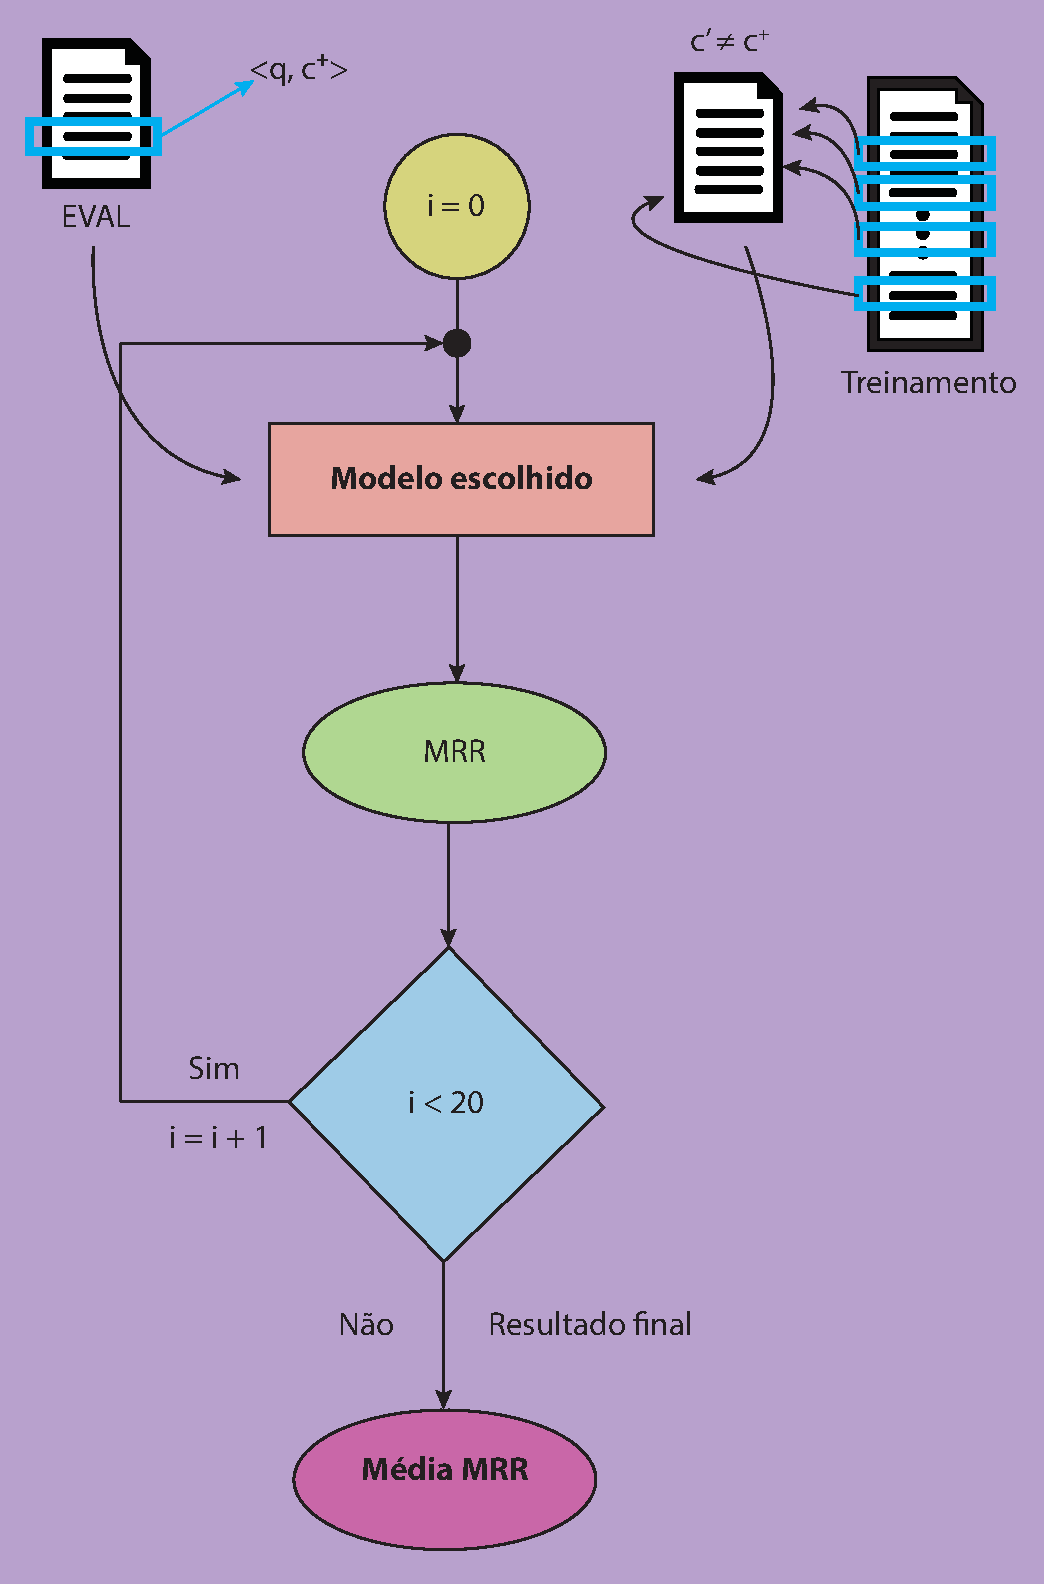
\includegraphics[height=1\textwidth]{figuras/cap-experimento/final_evaluation_process.pdf}
\caption{Ilustração do procedimento de avaliação proposto por \cite{iyer-etal-2016-summarizing}. O modelo com a maior média MRR no treinamento é avaliado na amostra EVAL. Durante 20 iterações, calculamos o MRR para os pares $<q, c^{+}>$ junto com outros 49 $c^{'}$ distratores, que são escolhidos da amostra de treinamento. Onde $q, c^{+}, c^{'} \in \mathbb{R}^{150 X d}$, tal $c^{+} \neq c^{'}$. A cada iteração outros 49 distratores $c^{'}$ são escolhidos. E ao final, obtemos o resultado do modelo.}
\label{fig:final-evaluation-process}
\end{figure}



\subsection{Arquiteturas}

Para este estudo, comparamos a arquitetura CNN com outras duas arquiteturas: \textit{Unif} e \textit{Embedding}. A arquitetura \textit{Unif} proposta por \cite{cambronero-deep-learning-code-search:2019} utiliza duas abordagens diferentes para representação das questões e trechos de código-fonte. No caso das questões, os vetores de representação distribuída de cada palavra são combinados através de uma média aritmética simples. Quanto aos trechos de código, aplica-se o \gls{mecanismo-atencao} que calcula uma média ponderada sobre os vetores de representação distribuída e aprende a ``prestar atenção`` nas palavras mais importantes.  Já a arquitetura \textit{Embedding} combina os vetores de representação distribuída de cada palavra através de uma camada \textit{max pool}. As figuras~\ref{fig:cnn-architecture}, \ref{fig:unif-architecture} e \ref{fig:embedding-architecture} ilustram as arquiteturas utilizadas.
\begin{figure}[h]
    \centering
    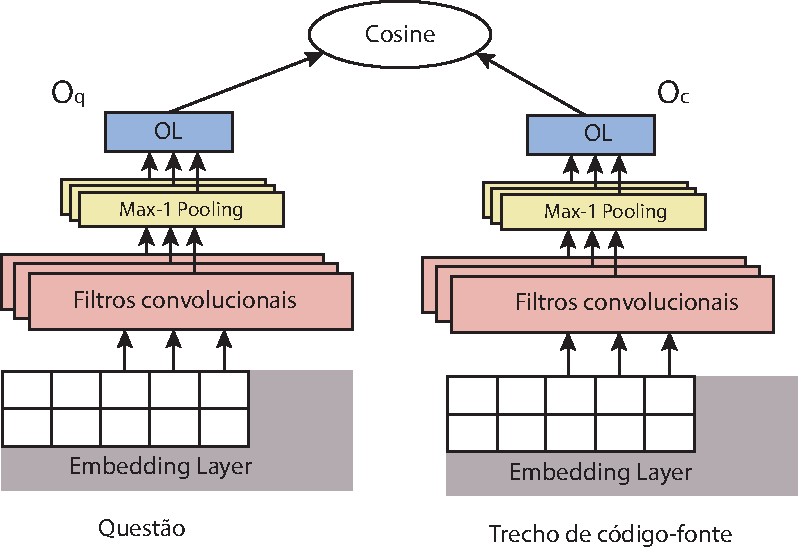
\includegraphics[width=0.8\textwidth]{figuras/cap-experimento/cnn-architecture-proposal.pdf}
    \caption{Figura da arquitetura CNN descrita no Capítulo~\ref{cap:abordagem}. O termo \emph{Embedding Layer} refere-se a camada composta por vetores de representação distribuída. OL é o acrônimo de \emph{Output Layer}, i.e., camada de saída. $O_{q}$ e $O_{c}$ indicam a saída do vetor de representação final das questões e trechos de código-fonte, respectivamente. \emph{Cosine} indica a função de similaridade.}
    \label{fig:cnn-architecture}
\end{figure}

\begin{figure}[h]
    \centering
    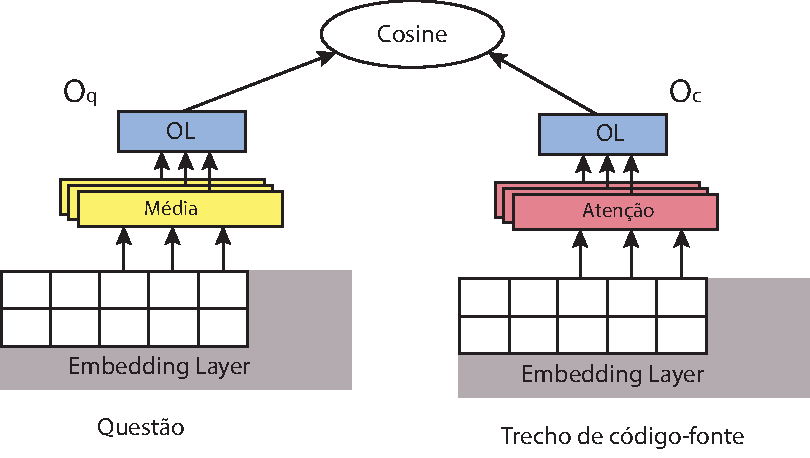
\includegraphics[width=0.8\textwidth]{figuras/cap-experimento/unif-architecture.pdf}
    \caption{Figura da arquitetura \Gls{unif} proposta por \cite{cambronero-deep-learning-code-search:2019}. \emph{Embedding} refere-se a camada composta pelos vetores de representação distribuída. \emph{Média} é camada que combina os vetores através de uma média aritmética simples. \emph{Atenção} refere-se ao \gls{mecanismo-atencao}, que combina os vetores através de uma média ponderada e aprende a ''prestar atenção'' nos termos mais relevantes. \emph{OL} é o acrônimo de \emph{Output Layer}, i.e., camada de saída. $O_{q}$ e $O_{c}$ referem-se ao vetor de representação final das questões e trechos de código, respectivamente. \emph{Cosine} indica a função de similaridade. }
    \label{fig:unif-architecture}
\end{figure}

\begin{figure}[h]
    \centering
    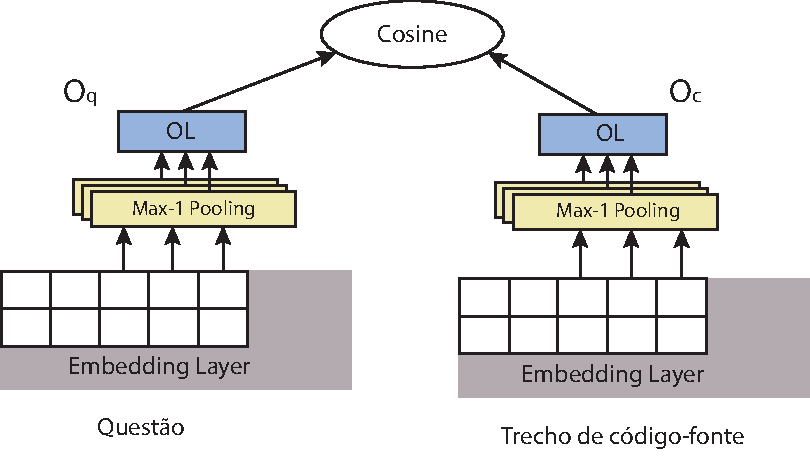
\includegraphics[width=0.8\textwidth]{figuras/cap-experimento/embedding-architecture.pdf}
    \caption{Figura da arquitetura de referência \textit{Embedding} para comparação. \emph{Embedding Layer} refere-se a camada composta pelos vetores de representação distribuída. \emph{OL} é o acrônimo de \emph{Output Layer}, i.e., camada de saída. $O_{q}$ e $O_{c}$ referem-se aos vetores de representação final das questões e trechos de código, respectivamente. \emph{Cosine} refere-se a função de similaridade. Figura utilizada no artigo \cite{marcelo-vem-2019}.}
    \label{fig:embedding-architecture}
\end{figure}
Nas figuras \ref{fig:cnn-architecture}, \ref{fig:unif-architecture} e \ref{fig:embedding-architecture}, a palavra \textit{Embedding Layer} refere-se ao vetor de representação distribuída das palavras. \emph{OL} é um acrônimo de \textit{Output Layer} ou camada de saída. $O_{q}$ indica a camada de saída da questão. $O_{c}$ indica a camada de saída do trecho de código-fonte. As arquiteturas CNN e \textit{Embedding} utilizam uma camada \textit{max pool}. E todas, ao final, calculam a similaridade atravás da função \textit{cosine}. Os ajustes dos hiper-parâmetros são discutidos com mais detalhes no Apêndicê~\ref{ape:ajuste-hiper-parametros-cnn} e no Capítulo~\ref{cap:resultados}, que também apresenta os resultados dos experimentos.

